
	\documentclass{article}
	\usepackage{amsmath,amssymb}
	\usepackage[inline]{enumitem}
	\usepackage{blindtext}
	\usepackage{booktabs}
	\usepackage{graphicx}
	\usepackage{xcolor}
	\usepackage[vmargin = 1.5in, top = 1in, bottom = 1.2in, letterpaper]{geometry}
	\usepackage{listings}
	\usepackage{courier}
	\usepackage{multicol}
	\usepackage{multirow}
	\lstset{
	basicstyle = \small\tt,
	keywordstyle = \tt\color{blue},
	commentstyle = \it\color[cmyk]{1,0,1,0},
	stringstyle = \tt\color[RGB]{128,0,0},
	%frame = single,
	backgroundcolor = \color[RGB]{245,245,244},
	breaklines,
	extendedchars = false,
	xleftmargin = 2em,
	xrightmargin = 2em,
	aboveskip = 1em,
	tabsize = 4,
	showspaces = false
	}
	\begin{document}
	
	% \newfontfamily\courier{Courier New}

	
	\title{STAT 542 Homework 6}
	\author{Yifan Zhu}
	\maketitle
	
	\begin{enumerate}[leftmargin = 0 em, label = \arabic*., font = \bfseries]
	\item 
	\begin{enumerate}
		\item When $\theta$ is the location parameter, denote $F(x)$ is the cdf with $\theta = 0$, i.e. $F(x) = F(x|0)$. Then $F(x|\theta) = F(x - \theta)$. cdf is non-decreasing, thus for $\theta_1 > \theta_2$ and any $x \in \mathbb{R}$, we have $x - \theta_1 < x - \theta_2$ and $F(x - \theta_1) \leq F(x - \theta_2)$. Hence, $F(x | \theta_1) \leq F(x|\theta_2)$, a location family is stochastically ordered in terms of location family.

		\item When $\theta$ is the scale parameter, denote $F(x)$ is the cdf with $\theta = 0$, i.e. $F(x) = F(x|0)$. Then $F(x|\theta) = F(x/\theta)$. cdf is non-decreasing, thus for $\theta_1 > \theta_2 > 0$ and any $x \in [0, \infty)$, we have $x / \theta_1 < x - \theta_2$ and $F(x / \theta_1) \leq F(x / \theta_2)$. For $x < 0$, we have $F(x) = 0$, thus $F(x / \theta_1) = F(x / \theta_2) = 0$. Hence, $F(x | \theta_1) \leq F(x|\theta_2),\, x \in \mathbb{R}$, a scale family is stochastically ordered in terms of location family.

	\end{enumerate}

	\item 
	\begin{enumerate}
		\item Let $D = \{(x,y)| x^2 + y^2 < 1\} \cap (-1,1)\times (-1,1) = \{(x,y)| x^2 + y^2 < 1\}$. Then
		\[P(X^2 + Y^2 < 1) = \iint_{D} \frac{1}{4} \mathrm{d}x \mathrm{d}y = \frac{\pi}{4}\]
		\begin{center}
		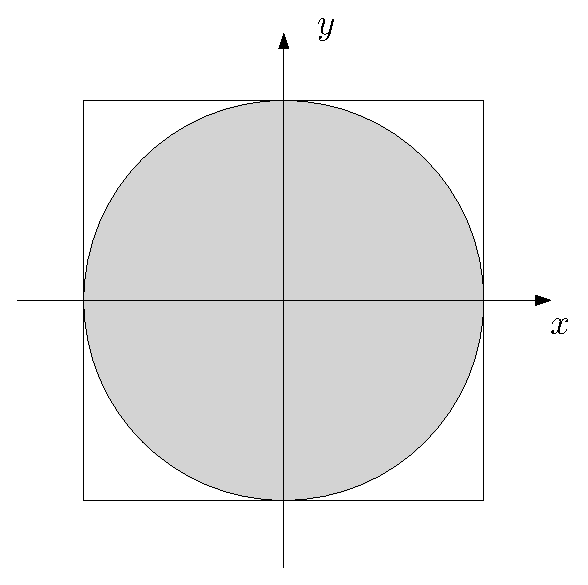
\includegraphics[width = 0.4\textwidth]{2a.eps}
		\end{center}

		\item Let $D = \{(x,y)| 2 x - y > 0\} \cap (-1,1)\times (-1,1) $. Then by symmetric
		\[P(2X - Y > 0) = \iint_{D} \frac{1}{4} \mathrm{d}x \mathrm{d}y = \frac{1}{2}\]
		\begin{center}
		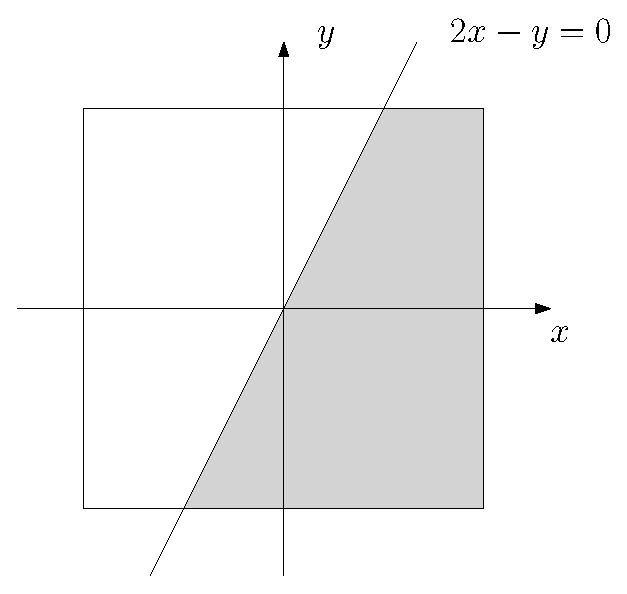
\includegraphics[width = 0.4\textwidth]{2b.eps}

		\item Let $D = \{(x,y)| x + y < 2\}\cap \{(x,y)| x + y > -2\} \cap (-1,1)\times (-1,1) = (-1,1)\times (-1,1)$. Then
		\[P(|X + Y| < 2) = \iint_{D} \frac{1}{4} \mathrm{d}x \mathrm{d}y = 1\]
		\begin{center}
		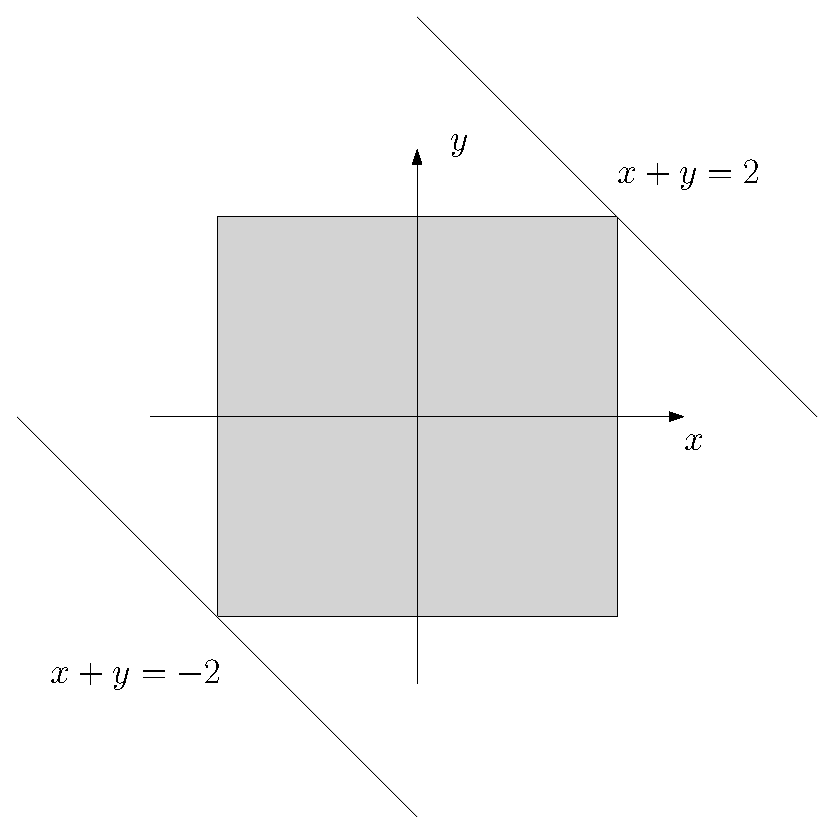
\includegraphics[width = 0.5\textwidth]{2c.eps}


		\end{center}


		\end{center}
	\end{enumerate}

	\item 
	\begin{enumerate}
		\item \begin{align*}
		&\int_{0}^1 \int_0^2 C(x + 2y) \mathrm{d}x \mathrm{d}y\\
		=& C\left( \left.\frac{1}{2} x^2 + 2 y x \right|_0^2\right)\mathrm{d}y\\
		=& C\left( 2 + 4y\right)\mathrm{d}y\\
		=& C\left(\left. 2y + 2y^2 \right|_0^1\right)\\
		=& 4C = 1 \qquad \Rightarrow C = \frac{1}{4}
		\end{align*}
		
		\item 
		\begin{align*}
		f_X(x) &= \int_0^1 \frac{1}{4}(x+ 2 y ) \mathrm{d}y\\
		& =  \frac{1}{4}\left( x y + y^2 \big|_0^1\right)\\
		& = \frac{1}{4}(x+1)
		\end{align*}

		\item 
		For $(x,y)\in \{(x,y)| x \leq 0\} \cup \{(x,y)| y\leq 0\}$, $F(x,y) = 0$.

		For $(x,y) \in \{(x,y)| x \geq 2\} \cup \{(x,y)| y \geq 1\}$, $F(x,y) = 1$.

		For $(x,y) \in \{(x,y)| 0< x < 2\} \cap \{(x,y)| 0 < y < 1\}$, $F(x,y) = \int_0^y \int_0^x \frac{1}{4}(s + 2t) \mathrm{d}s \mathrm{d}t = \frac{1}{8} x^2 y + \frac{1}{4}xy^2$.

		For $(x,y) \in \{(x,y)| 0 < x < 2\} \cap \{(x,y)| y \geq 1\}$, $F(x,y) = \int_{0}^1 \int_0^x \frac{1}{4}(s+ 2t)\mathrm{d}s \mathrm{d}t = \frac{1}{8}x^2 + \frac{1}{4}x $.

		For $(x,y) \in \{(x,y)| x \geq 2\} \cap \{(x,y)| 0 < y < 1\}$, $F(x,y) = \int_{0}^y \int_0^2 \frac{1}{4}(s+ 2t)\mathrm{d}s \mathrm{d}t = \frac{1}{2}y^2 + \frac{1}{2} y$.

		\item  $g(x) = \frac{9}{(x+1)^2}$ is monotone on $(0, 2)$. Support of $Z$ is then $(1, 9)$.  $g^{-1}(z) = \frac{3}{\sqrt{z}} - 1,\, \left|\frac{\mathrm{d}}{\mathrm{d}z}g^{-1}(z)\right| = \frac{3}{2} z^{-3/2}.$ Thus 
		\[f_Z (z) = f_X(g^{-1}(z)) \left|\frac{\mathrm{d}}{\mathrm{d}z}g^{-1}(z)\right| = \frac{9}{8}z^{-2}, \, 1< z < 9\]

		
	\end{enumerate}
	

	\item 
	\begin{enumerate}
		\item \begin{align*}
		P(X > \sqrt{Y}) & = \int_{0}^1 \int_{0}^{x^2} (x+y)\mathrm{d}y \mathrm{d}x\\
		& = \int_0^1 (x^3 + \frac{1}{2} x^4) \mathrm{d}x\\
		& = \frac{1}{4}x^4 + \frac{1}{10} x^5 \bigg|_0^1 \\
		& = \frac{7}{20}
		\end{align*}
		
		\item \begin{align*}
		P(X^2 < {Y} < X) & = \int_{0}^1 \int_{x^2}^{x} 2x \mathrm{d}y \mathrm{d}x\\
		& = \int_0^1 2x(x - x^2) \mathrm{d}x\\
		& = \frac{2}{3}x^3 + \frac{1}{2} x^4 \bigg|_0^1 \\
		& = \frac{1}{6}
		\end{align*}
	\end{enumerate}


	\item 
	\begin{enumerate}
		\item $f(x,y) = P(X = x, Y = y)$. Then $f(1,3) = 1/12,\, f(1,5) = 1/12,\, f(1,8) = 1/12,\, f(3,3) = 1/12,\, f(3,5) = 1/12,\, f(3,8) = 1/12,\, f(5,5) = 2/12 = 1/6,\, f(5,8) = 1/12,\, f(8,8) = 3/12 = 1/4.$ For other $(x,y)$, $f(x,y) = 0$.
\begin{center}
		\begin{tabular}{c|ccccc}
                   &   & \multicolumn{4}{c}{$x$}    \\
                   \hline
                   &   & 1    & 3    & 5    & 8   \\
\multirow{3}{*}{$y$} & 3 & 1/12 & 1/12 & 0    & 0   \\
                   & 5 & 1/12 & 1/12 & 1/6  & 0   \\
                   & 8 & 1/12 & 1/12 & 1/12 & 1/4
\end{tabular}
\end{center}

		\item $f_X (1) = f(1,3) + f(1,5) +f(1,8) = 3/12 = 1/4,\, f_X(3) = f(3,3) + f(3,5) +f(3,8) = 3/12 = 1/4,\, f_X(5) = f(5,5) + f(5,8) = 1/6 + 1/12 = 1/4,\, f_X(8) = 1/4$. For other $x$, $f_X(x) = 0$.

		\begin{center}
\begin{tabular}{c|cccc}
$x$ & 1   & 3   & 5   & 8   \\
\hline
  & 1/4 & 1/4 & 1/4 & 1/4
\end{tabular}
		\end{center}

		$f_Y (3) = f(1,3) + f(3,3) = 2/12 = 1/6,\, f_X(5) = f(1,5) + f(3,5) +f(5,5) = 2/12 + 1/6 = 1/3,\, f_X(8) = f(1,8) + f(3,8) + f(5,8) + f(8,8)= 3/12 + 1/4 = 1/2 $. For other $y$, $f_Y(y) = 0$.

		\begin{center}
\begin{tabular}{c|cccc}
$y$ &  3   & 5   & 8   \\
\hline
  & 1/6 & 1/3 & 1/2 
\end{tabular}
		\end{center}

		\item $E(X) = 1 \cdot f_X(1) + 3 \cdot f_X (3) + 5 \cdot f_X(5) + 8 \cdot f_X(8) = \frac{17}{4}$.

		$E(Y - X) = 2 \cdot f(1,3) + 4 \cdot f(1,5) + 7 \cdot f(1,8) + 2 \cdot f(3,5) + 5 \cdot f(3,8) + 3 \cdot f(5,8) = \frac{23}{12}$


		\item $E(Y) = 3f_Y(3) + 5f_Y(5) + 8f_Y(8) = 1/2 + 5/3 + 4 = \frac{37}{6}$.

		$E(XY) = 3 f(1,3) + 5 f(1,5) + 8 f(1,8) + 9 f(3,3) + 15 f(3,5) + 24 f(3,8) + 25 f(5,5) + 40 f(5,8) + 64 f(8,8) = \frac{173}{6}$.

		Then $Cov(X,Y) = E(XY) - E(X) E(Y) = 173/6 - (37/6) \cdot (17/4) = \frac{21}{8} = 2.625 $


	\end{enumerate}

	\item 
	\begin{align*}
	&Cov(X_1 - 2 X_2 + 8, 3 X_1 + X_2) \\
	=& 3 Cov(X_1, X_1) + Cov(X_1, X_2) - 6 Cov(X_1, X_2) - 2 Cov(X_2 , X_2)\\
	 =& 3 \sigma_1^2 - 5 \sigma_{12} - 2 \sigma_2^2
	\end{align*}


	\item 
	\begin{enumerate}
		\item If $P(X > Y) = 0$, then $E(X - Y) = \iint_{\mathbb{R}^2} (x - y) f(x, y)\mathrm{d}x \mathrm{d}y = \iint_{\{(x,y)|x \leq y\}} (x - y)f(x,y) \mathrm{d}x \mathrm{d}y \leq 0$. This contradicts the assumption that $EX > EY$. Thus when $EX > EY$, we have $P(X > Y) > 0$. 

		\item 
		$F(x,y) = \max\{F_X (x), F_Y (y)\}$ is not a legistimate cdf.

		 From the definition, we have $F(x,y) \geq F_X (x),\, F(x,y) \geq F_Y (y)$. For a fixed $y$ such that $F_Y(y) > 0$, let $x \to -\infty$, $\lim_{x\to -\infty} F(x,y) \geq \lim_{x \to -\infty} F_Y (y) = F_Y (y) > 0$. Thus $F(x,y)$ is not a legistimate cdf.


		 \item 
		 $F(x,y) = \min\{F_X (x), F_Y (y)\}$ is a legistimate cdf.

		 $g(x,y) = \min\{x, y\}$ is a continuous function for $(x,y)$ in $\mathbb{R}^2$. Thus we can take the limit inside.

		 \begin{enumerate}
		 	\item $\lim_{x \to -\infty} F(x,y) = \lim_{x\to -\infty}\min\{F_{X}(x), F_Y(y)\} = \min\{\lim_{x\to -\infty}F_{X}(x), \lim_{x\to -\infty} F_Y (y)\} = \min\{0, F_Y (y)\} = 0$.

		 	$\lim_{y \to -\infty} F(x,y) = \lim_{y\to -\infty}\min\{F_{X}(x), F_Y(y)\} = \min\{\lim_{y\to -\infty}F_{X}(x), \lim_{y\to -\infty} F_Y (y)\} = \min\{F_X (x), 0\} = 0$.


		 	\item 
		 	$\lim_{x,y \to \infty} F(x,y) = \lim_{x,y\to\infty}\min\{F_X (x), F_Y (y)\} = \min\{\lim_{x,y \to \infty} F_X (x) , \lim_{x,y \to \infty} F_Y (y)\} = \min\{1,1\} = 1$.

		 	\item 
		 	$\lim_{h \to 0^+} F(x + h , y) = \lim_{h \to 0^+} \min\{F_X(x + h), F_Y(y)\} = \min\{\lim_{h \to 0^+}F_{X}(x+h), \lim_{h \to 0^+}F_Y(y)\} = \min\{F_X(x), F_Y (y)\} = F(x,y)$. In the same way, we can prove $\lim_{h\to 0^+}F(x, y+h) = F(x,y)$. 

		 	\item When $F_Y(y) \leq F_X(x) \leq  F_X(x+ \Delta_1) \leq F_Y(y + \Delta_2) $, 

		 	$F(x+\Delta_1 , y + \Delta_2) - F(x+ \Delta_1,y) - F(x, y + \Delta_2) + F(x,y) = F_X (x +\Delta_1 ) - F_Y(y) - F_X (x) + F_{Y}(y) = F_X (x + \Delta_1) - F_X (x) \geq 0$.

		 	\

		 	When $F_X(x) \leq F_Y(y) \leq  F_Y(y+ \Delta_2) \leq F_X(x + \Delta_1) $, 

		 	$F(x+\Delta_1 , y + \Delta_2) - F(x+ \Delta_1,y) - F(x, y + \Delta_2) + F(x,y) = F_Y (y +\Delta_2 ) - F_Y(y) - F_X (x) + F_{X}(x) = F_Y (y + \Delta_2) - F_Y (y) \geq 0$.

		 	\

		 	When $F_X(x) \leq F_Y(y) \leq  F_X(x+ \Delta_1) \leq F_Y(y + \Delta_2) $, 

		 	$F(x+\Delta_1 , y + \Delta_2) - F(x+ \Delta_1,y) - F(x, y + \Delta_2) + F(x,y) = F_X (x +\Delta_1 ) - F_{Y}(y) - F_X (x) + F_{X}(x) = F_X (x + \Delta_1) - F_Y (y) \geq 0$.

		 	\

		 	When $F_Y(y) \leq F_X(x) \leq  F_Y(y + \Delta_2) \leq F_X(x + \Delta_1) $, 

		 	$F(x+\Delta_1 , y + \Delta_2) - F(x+ \Delta_1,y) - F(x, y + \Delta_2) + F(x,y) = F_Y (y +\Delta_2 ) - F_Y(y) - F_X (x) + F_{Y}(y) = F_Y (y + \Delta_2) - F_X (x) \geq 0$.

		 	\

		 	When $F_Y(y) \leq F_Y(y + \Delta_2) \leq  F_X(x) \leq F_X(x + \Delta_1) $, 

		 	$F(x+\Delta_1 , y + \Delta_2) - F(x+ \Delta_1,y) - F(x, y + \Delta_2) + F(x,y) = F_Y (y +\Delta_2 ) - F_Y(y) - F_Y (y + \Delta_2) + F_{Y}(y) =  0$.

		 	\

		 	When $F_X(x) \leq F_X(x + \Delta_1) \leq  F_Y(y) \leq F_Y(y + \Delta_2) $, 

		 	$F(x+\Delta_1 , y + \Delta_2) - F(x+ \Delta_1,y) - F(x, y + \Delta_2) + F(x,y) = F_X (x +\Delta_1 ) - F_X(x) - F_X (x + \Delta_1) + F_{X}(x) =  0$.

		 	Thus in any situation, we all have 
		 	\[F(x+\Delta_1 , y + \Delta_2) - F(x+ \Delta_1,y) - F(x, y + \Delta_2) + F(x,y) = F_X (x +\Delta_1 ) - F_X(x) - F_X (x + \Delta_1) + F_{X}(x) \geq  0\]

		 	Thus $F(x,y) = \min\{F_X(x), F_Y (y)\}$ is a legistimate cdf.





		 \end{enumerate}
		 



		 


	\end{enumerate}
	
	
	
	
	
	
	
	
 	\end{enumerate}


	
	
	
	\end{document}